% =====================================================================
% Diagrama de sequência --- Iago (Frente 3)
% Só o Iago edita este arquivo. Salve a imagem em figuras/ e o código-fonte
% (PlantUML) em documentos/uml/.
% =====================================================================
\section{Diagrama de sequência}\label{sec:sequencia}

A Figura~\ref{fig:sequencia} mostra as mensagens trocadas quando o usuário pede o ranking de
influenciadores da Twitch PT (caso de uso UC14, que inclui o UC09, calcular centralidades). O
fluxo passa por quatro camadas: usuário, interface, centralidades e grafo.

\begin{figure}[htbp]
\centering
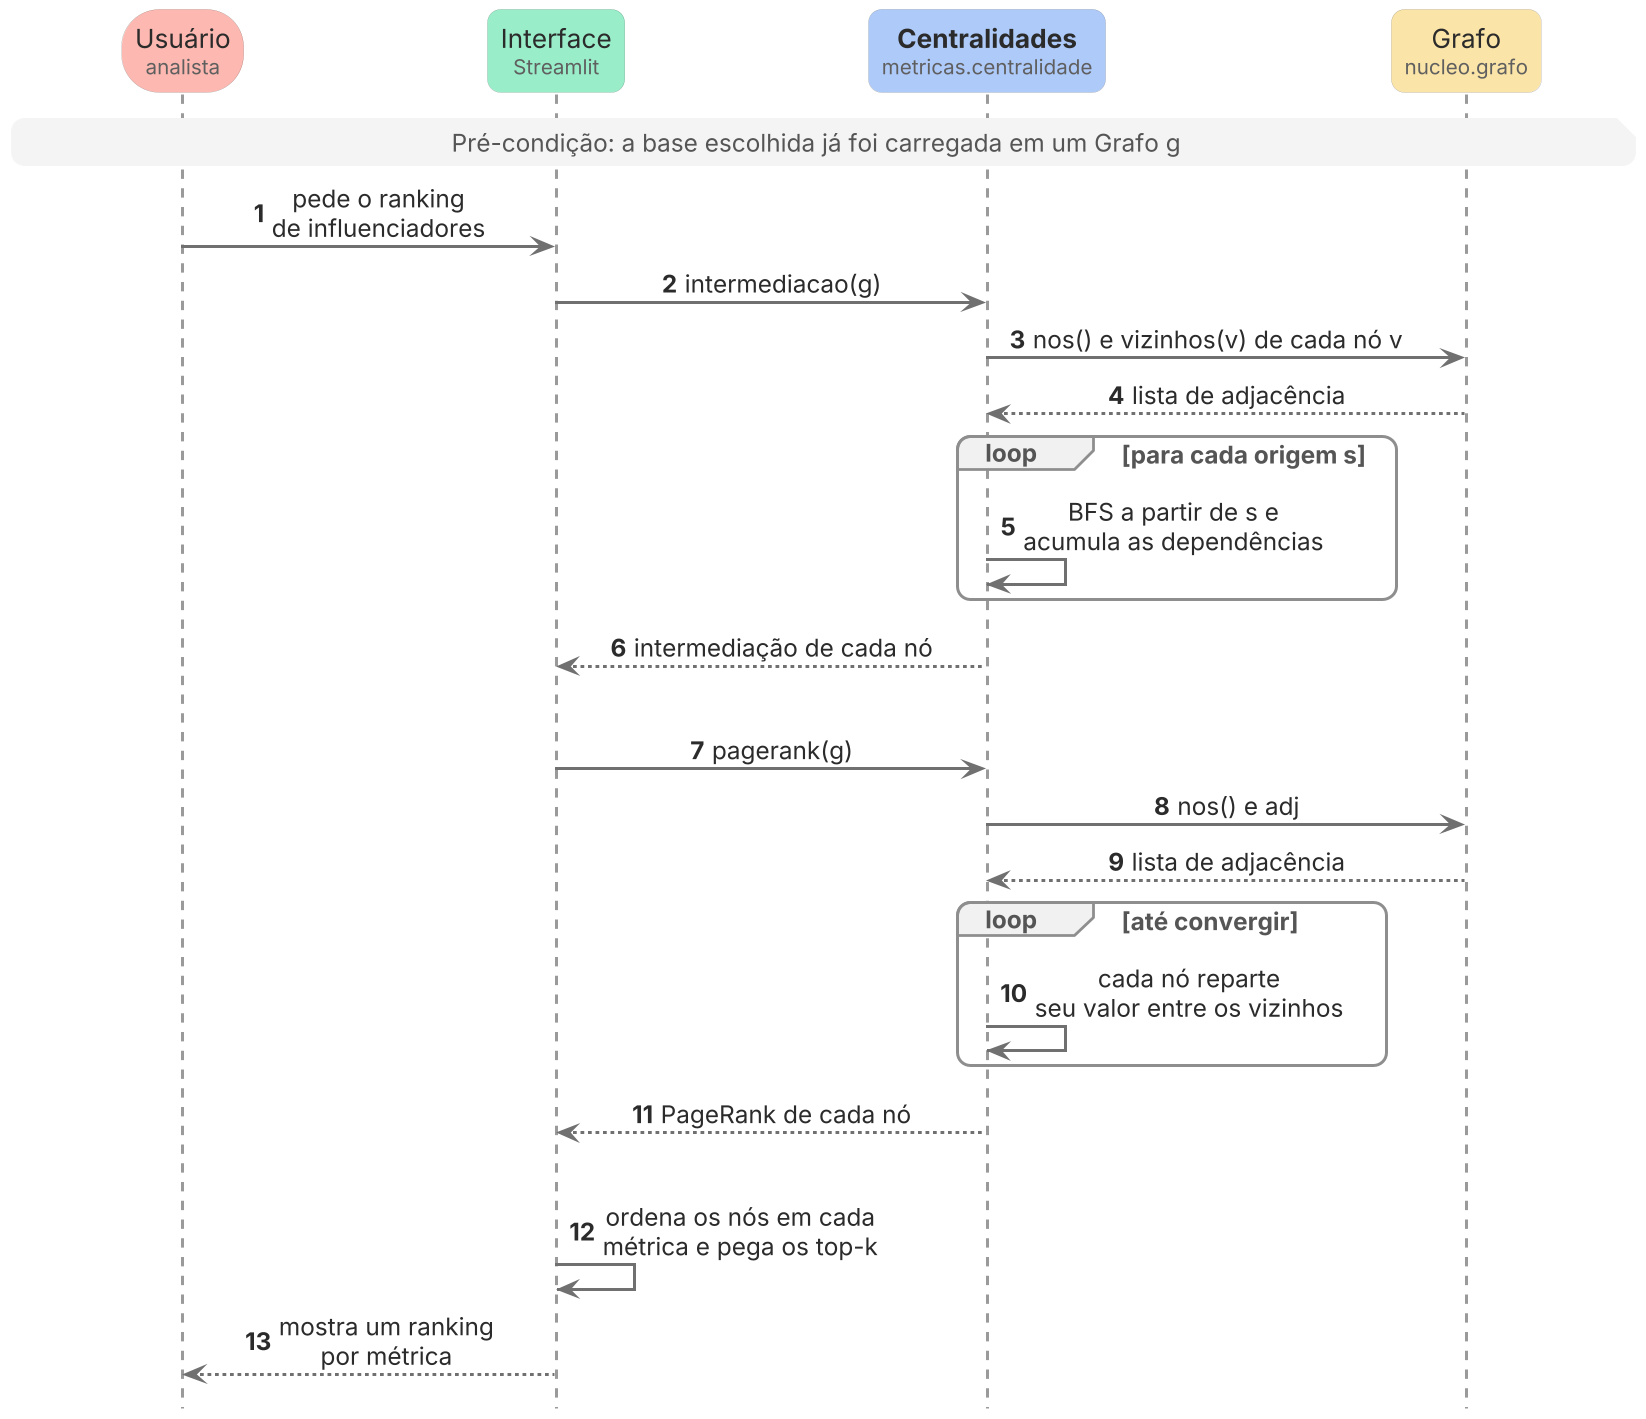
\includegraphics[width=\textwidth]{sequencia.png}
\caption{Diagrama de sequência do ranking de influenciadores.}
\label{fig:sequencia}
\end{figure}

O diagrama parte de um grafo já carregado. Quando o usuário pede o ranking (mensagem 1), a
interface chama \codigo{intermediacao(g)} (mensagem 2). A função lê os nós e os vizinhos do
grafo uma única vez, em $O(n + m)$, e monta uma lista de adjacência indexada por inteiros
(mensagens 3 e 4). Depois, o algoritmo de Brandes~\cite{brandes2001} faz uma busca em largura a
partir de cada origem $s$, conta os caminhos mínimos que saem de $s$ e acumula a parcela de
cada nó nesses caminhos (mensagem 5), sem voltar a consultar o grafo. Como são $n$ buscas de
custo $O(n + m)$, o total é $O(nm)$; na versão por amostragem, só $k$ origens sorteadas entram
no laço, em $O(km)$, e o resultado é multiplicado por $n/k$ para estimar o valor
exato~\cite{brandes2007}. A função devolve um valor por nó (mensagem 6). O
\codigo{pagerank(g)} segue o mesmo padrão: lê a adjacência uma vez (mensagens 8 e 9) e repete
a distribuição dos valores entre os vizinhos até convergir (mensagem 10). O k-core
(\codigo{numero\_de\_nucleo}), a terceira centralidade da Frente 3, segue o mesmo padrão (lê o
grafo uma vez e calcula sobre a lista indexada) e foi omitido para o diagrama não ficar longo.
Por fim, a interface ordena os nós em cada métrica, pega os $k$ primeiros e mostra um ranking por métrica
(mensagens 12 e 13). As métricas não são somadas: comparar os rankings entre si e com o alcance
na simulação SIR é o papel do módulo \codigo{aplicacao} (Seção~\ref{sec:problema}). As
centralidades só chamam métodos de consulta do \codigo{Grafo} e nunca o alteram, como exigem as
regras do grupo.
